\documentclass[a4paper,12pt]{article}
\usepackage[utf8x]{inputenc}
\usepackage{amssymb}
\usepackage{amsfonts}
\usepackage{mathrsfs}
\usepackage{amsmath}
\usepackage{amsthm}
\usepackage[margin=3cm]{geometry}
\usepackage{times}
\usepackage{graphicx}
\usepackage{enumitem}
\usepackage{fancyhdr}
\usepackage{hyperref}
\usepackage{setspace}
\usepackage{subcaption}
\usepackage{mathtools}

\usepackage{lineno}
\linenumbers
\renewcommand{\baselinestretch}{1.5}
\usepackage{authblk}

\newtheorem{theorem}{Theorem}
\newtheorem{proposition}{Proposition}[section]
\newtheorem{lemma}{Lemma}[section]
\newtheorem{corollary}{Corollary}[section]
\theoremstyle{definition}
\newtheorem{definition}{Definition}[section]

\newcommand{\boldnabla}{\mbox{\boldmath$\nabla$}} % to be used in mathmode
\newcommand{\cbar}{\overline{\mathbb{C}}}% to be used in mathmode
\newcommand{\diff}[2]{\frac{d #1}{d #2}}% to be used in mathmode
\newcommand{\difff}[2]{\frac{d^2 #1}{d #2^2}}% to be used in mathmode
\newcommand{\pdiff}[2]{\frac{\partial #1}{\partial #2}} % to be used in mathmode
\newcommand{\pdifff}[2]{\frac{\partial^2 #1}{\partial #2^2}}% to be used in mathmode
\newcommand{\upperth}{$^{\mbox{\footnotesize{th}}}$}%to be used in text mode
\newcommand{\vect}[1]{\mathbf{#1}}% to be used in mathmode
\newcommand{\curl}[1]{\boldnabla \times \vect{#1}} % to be used in mathmode
\newcommand{\divr}[1]{\boldnabla \cdot \vect{#1}} %to be used in mathmode
\newcommand{\modu}[1]{\left| #1 \right|} %to be used in mathmode
\newcommand{\brak}[1]{\left( #1 \right)} % to be used in mathmode
\newcommand{\comm}[2]{\left[ #1 , #2 \right]} %to be used in mathmode
\newcommand{\dop}{\vect{d}} %to be used in mathmode
\newcommand{\cov}{\text{cov}} %to be used in mathmode
\newcommand{\var}{\text{var}} %to be used in mathmode
\newcommand{\mb}{\mathbf} %to be used in mathmode
\newcommand{\bs}{\boldsymbol} %to be used in mathmode
% Title Page
\title{Functional networks expand across anatomical boundaries as correlation time-scale increases}
\date{}

\author[1]{Thomas Delaney}
\author[2]{Michael C. Ashby}
\author[1]{Cian O'Donnell}
\affil[1]{School of Computer Science, Electrical and Electronic Engineering, and Engineering Mathematics, University of Bristol, Bristol, United Kingdom.}
\affil[2]{School of Physiology, Pharmacology and Neuroscience, University of Bristol, Bristol, United Kingdom.}
\renewcommand\Affilfont{\itshape\small}

\begin{document}

\maketitle

%\tableofcontents

\abstract{Decades of research has established that correlations play a crucial role in representing sensory information. One drawback associated with the recent improvement in recording technology and consequent large datasets is the difficulty in analysing higher order correlations in large neuronal ensembles. One benefit of these datasets that has not yet been explored is the opportunity to compare correlations within anatomical regions to correlations across anatomical regions. In this work, we measured correlations between neurons residing in nine different brains regions in three awake and behaving mice. Using the these correlation measurements, we created weighted undirected graph networks and applied network science methods to detect functional communities in our neural ensembles. We compared these functional communities to their anatomical distribution. We repeated the analysis, using different timescales for our correlation measurements, and found that functional communities were more likely to be dominated by neurons from a single brain region at shorter timescales ($< 100$ms).}

\section{Introduction}
Decades of research has established that correlations play a crucial role in representing sensory information. For example, the onset of visual attention has been shown to have a greater affect on the correlations in the macaque V4 region than on the firing rates in that region \cite{cohen1}. Recent findings show that spontaneous behaviours explain correlations in parts of the brain not associated with motor control \cite{stringer}. In order to understand the brain, we must understand the interactions between neurons.

Because of limitations in recording technology almost all research has explored correlations between neurons within a given brain region. Relatively little is known about correlations between neurons in different brain regions. However, the recent development of `Neuropixels' probes \cite{jun} has allowed extracellular voltage measurements to be collected from multiple brain regions simultaneously routinely, and in much larger numbers than traditional methods. In this project we used a publicly-available Neuropixels dataset to analyse correlations between different brain regions \cite{stringer}.

A drawback associated with the improvement in recording technology is an increase in the difficulty of analysing these data. For example, analysing the $i$th order interactions of $N$ neurons generally requires estimation of $N^i$ parameters. A number that becomes astronomical for large $N$. New methods are required for analysing these new large datasets. We attempted to address this requirement in this piece of research by applying a cutting-edge network science community detection method to neural data.

Another unexplored area of research is the changes in cell interactions at different timescales. Most studies focus on quantifying interactions at a given timescale. But neurons may interact differently, or may interact with different neurons, at different timescales. Here we explore correlated communities of neurons at different timescales.

In this work, we measured spike count correlations between neurons from nine different regions of the mouse brain. Using these correlation measurements, we created weighted undirected graphs or networks with each node representing a neuron. We used newly invented network methods to detect communities in these networks. We compared these detected communities to the anatomical division of the cells. We also measured the conditional correlation and signal correlation of between cell spike counts, conditioning on the subjects' behaviour. We repeated the network analysis using these measurements. We also repeated these analyses using different timescales for measuring the correlations.

\section{Results}

    \subsection{Average correlation size increases with increasing time bin width}
    First we inspected the affect of time bin width on spike count correlations. We know that using short time bins results in artificially small correlation measurements\cite{cohen2}, so we expected to see an increase in correlation amplitude with increasing time bin width. That is exactly what we observed. Taking $50$ cells at random, we calculated the spike count correlation between every possible pair of these cells, using different time bin widths ranging from $0.005$s to $3$s. We found that the longer the time bin width, the greater the correlations (see figure \ref{fig:correlations_all_pairs}).

    We also separated the positively correlated pairs from the negatively correlated pairs using the mean correlation of each pair across all bin widths (see section \ref{sec:corr_anti_corr}). We found that the positively correlated pairs become more positively correlated with increasing time bin width, and the negatively correlated pairs become more negatively correlated with increasing time bin width (see figures \ref{fig:correlations_pos_pairs} and \ref{fig:correlations_neg_pairs}).

    When taking the mean across all pairs, the positively correlated pairs dominate in terms of both number of pairs, and amplitude of correlations. Therefore the mean across all pairs is positive.

    These results were observed in each of the three mouse subjects from which we had data.

    \subsection{Goodness-of-fit for Poisson and Gaussian distributions across increasing time bin widths}
    We wanted to investigate if the width of the time bin used to bin spike times into spike counts had an effect on the distribution of spike counts.  We used the $\chi^2$ statistic as a goodness-of-fit measure for Poisson and Gaussian (normal) distributions to the spike count of $100$ randomly chosen neurons for a number of bin widths ranging from $0.01$s to $4$s. For the $\chi^2$ statistic, the higher the value, the worse the fit. As you might expect, we found that that a Poisson distribution is the best fit for shorter time bins less than $0.7$s in length. Then a Gaussian distribution is a better fit for time bins greater than $0.7$s in length (see figure \ref{fig:chi_squared_fits}).

    A Poisson distribution was very likely to be a better fit for shorter time bin widths because spike counts must be non-negative, therefore any distribution of spike counts with mass distributed at or close to $0$ will be skewed.

    \begin{figure}[h]
        \begin{subfigure}[h]{0.5\linewidth}
            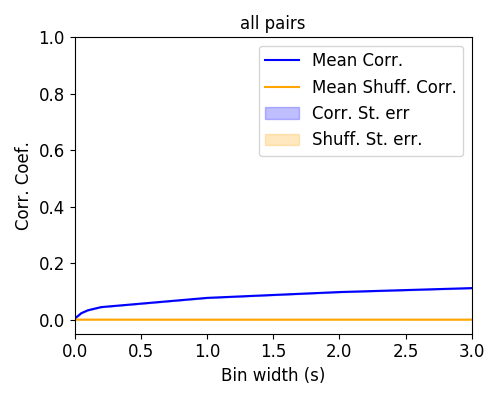
\includegraphics[width=\linewidth]{figures/Krebs_corr_all_pairs.png}
            \caption{All pairs, positive and negative.}
            \label{fig:correlations_all_pairs}
        \end{subfigure}
        \begin{subfigure}[h]{0.5\linewidth}
            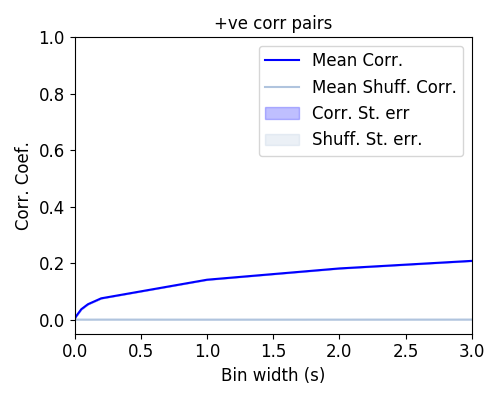
\includegraphics[width=\linewidth]{figures/Krebs_corr_pos_pairs.png}
            \caption{All positively correlated pairs.}
            \label{fig:correlations_pos_pairs}
        \end{subfigure}
        \begin{subfigure}[h]{0.5\linewidth}
            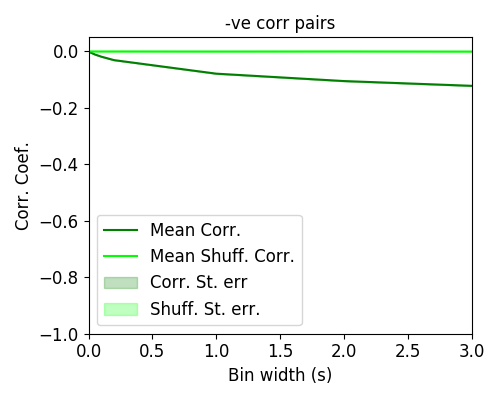
\includegraphics[width=\linewidth]{figures/Krebs_corr_neg_pairs.png}
            \caption{All negatively correlated pairs.}
            \label{fig:correlations_neg_pairs}
        \end{subfigure}
        \begin{subfigure}[h]{0.5\linewidth}
            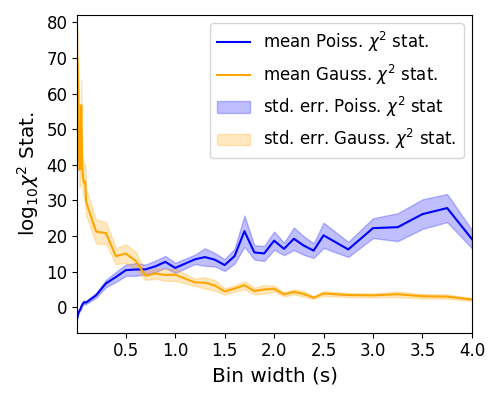
\includegraphics[width=\linewidth]{figures/Krebs_stats_by_bin_width.png}
            \caption{$\chi^2$ test statistics as goodness-of-fit.}
            \label{fig:chi_squared_fits}
        \end{subfigure}
        \caption{Mean correlation coefficients measured from pairs of $50$ randomly chosen neurons. (a) All possible pairs, (b) positively correlated pairs, and (c) negatively correlated pairs. (d) Mean and standard error of $\chi^2$ test statistics for Poisson and Gaussian distributions fitted to neuron spike counts.}
        \label{fig:correlations_vs_bin_widths}
    \end{figure}

% Fig 1. Correlations increase with bin width
% - 2 time series plots of a pair of neurons, one small bin width one big bin widt
%
  \subsection{Differences between and inter- and intra- regional correlations decrease with increasing bin width}
  We investigated the differences in distribution between inter-regional correlations, i.e. correlations between neurons in different brain regions, and intra-regional correlations, i.e. correlations between neurons in the same brain region.

  Firstly, we investigated these quantities for all possible pairs of $\sim 500$ neurons taken from across all the $9$ brain regions from which we had data. We distributed these neurons as evenly as possible across all of the regions, so that cell from one region would not dominate our data. We observed that the mean intra-regional correlations were always higher than the mean inter-regional correlations for every value of time bin width used. We also observed that as the time bin width increased these mean correlations increased and the difference between the mean inter-regional and intra-regional correlations grew (see figure \ref{fig:all_pairs_inter_intra_corr}). Stringer et al. (2019) had a similar finding using the same data. They used only one value for the time bin width, $1.2$s. Using this time bin width to bin spike times and measure spike count correlations, they found that the mean `within-region' correlations were always greater than the `out-of-region' correlations \cite{stringer}.

  \begin{figure}[h]
    \centering
    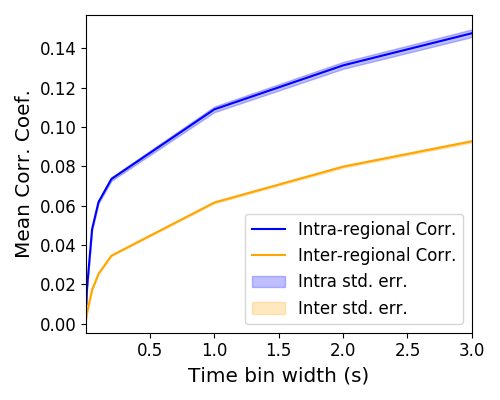
\includegraphics[width=0.5\linewidth]{figures/Krebs_inter_intra_regional_correlations.png}
    \caption{The mean intra-region and inter-region correlations using all possible pairs of $\sim 500$ neurons, spread across $9$ different brain regions.}
    \label{fig:all_pairs_inter_intra_corr}
  \end{figure}

  Secondly, we separated those pairs into theire respective pairs, be they intra-regional, or inter-regional.  We noted that the mean intra-regional correlations for a given region tended to be higher than the mean inter-regional correlations involving cells from that region. However, in contrast with our previous result, we noted that the difference between the mean intra-regional correlations and most mean inter-regional correlations of the most correlated regional pairs reduced as we increased the time bin width (see figures \ref{fig:short_bin_corr_comp} and \ref{fig:long_bin_corr_comp}).

  \newpage

  \begin{figure}[h]
    \begin{subfigure}[h]{\linewidth}
      \centering
      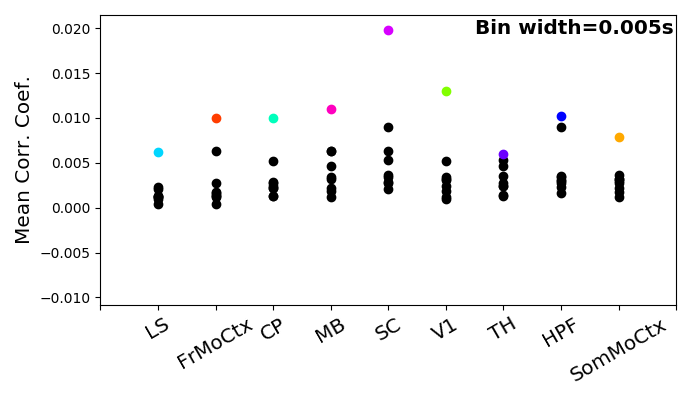
\includegraphics[width=0.7\linewidth]{figures/Krebs_0p005_corr_comp.png}
      \caption{Mean inter-regional and intra-regional correlations using a time bin width of 5ms.}
      \label{fig:short_bin_corr_comp}
    \end{subfigure}
    \begin{subfigure}[h]{\linewidth}
      \centering
      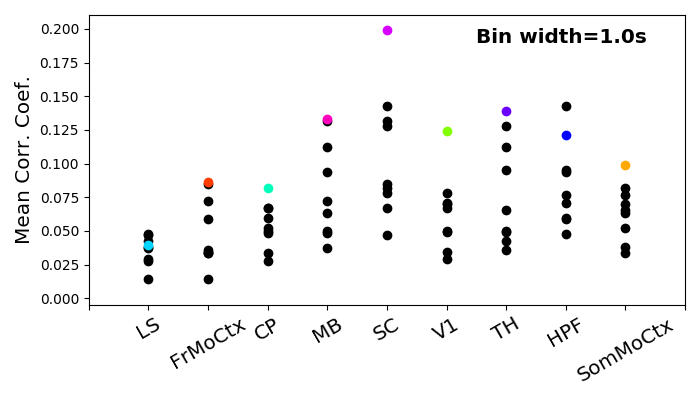
\includegraphics[width=0.7\linewidth]{figures/Krebs_1p0_corr_comp.png}
      \caption{Mean inter-regional and intra-regional correlations using a time bin width of 1s.}
      \label{fig:long_bin_corr_comp}
    \end{subfigure}
    \caption{The mean intra-regional correlations (coloured dots) and mean inter-regional correlations (black dots) for a given region, indicated on the x-axis, for different time bin widths. Each black dot represents the mean inter-regional correalations between the region indicated on the x-axis and one other region. (a) shows these measurements when we used a time bin width of 5ms. (b) shows these measurements when we used a time bin width of 1s. Note that the difference between the mean inter-regional correlations and mean intra-regional correlations is smaller for 1s bins.}
    \label{fig:corr_comps}
  \end{figure}

  Finally, to see these regional mean correlations in a bit more detail, we displayed these data using mean correlation matrix figures (see figure \ref{fig:corr_matrices}), showing the mean intra-regional correlations on the main diagonal, and the mean inter-regional correlations off diagonal. Comparing a version of this figure created using a short time bin width of $5$ms (figure \ref{fig:short_bin_corr_matrix}) and a version using a longer time bin width of $1$s (figure \ref{fig:long_bin_corr_matrix}) we observed that the mean intra-regional correlations are the highest for both bin widths, but the mean correlations in some inter-regional pairs is relatively much higher when using the longer time bin width.

  \begin{figure}[h]
    \begin{subfigure}[h]{0.5\linewidth}
      \centering
      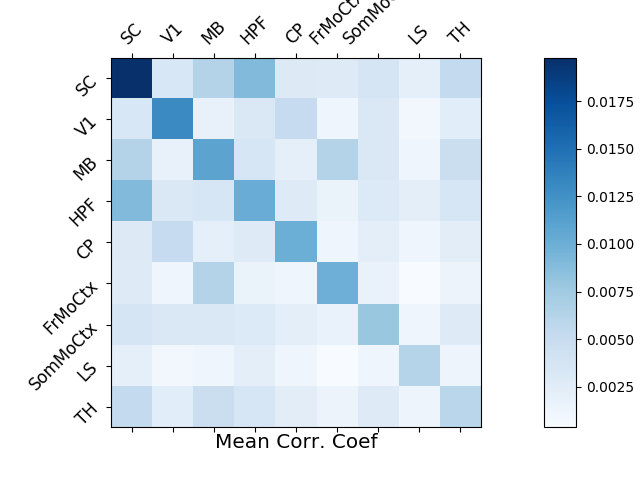
\includegraphics[width=\linewidth]{figures/Krebs_0p005_corr_matrix.png}
      \caption{Time bin width 0.005s.}
      \label{fig:short_bin_corr_matrix}
    \end{subfigure}
    \begin{subfigure}[h]{0.5\linewidth}
      \centering
      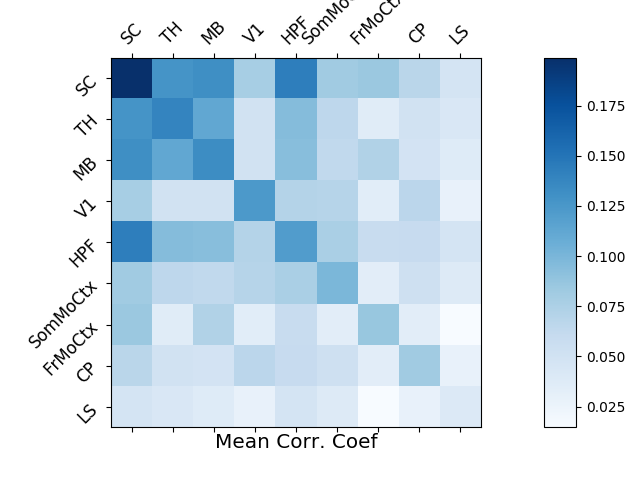
\includegraphics[width=\linewidth]{figures/Krebs_1p0_corr_matrix.png}
      \caption{Time bin width 1s.}
      \label{fig:long_bin_corr_matrix}
    \end{subfigure}
    \caption{Mean inter-regional (main diagonal) and intra-regional (off diagonal) correlation coefficients. (a) Shows these measurements when spike times were binned using $5$ms time bins. (b) Shows the same, using $1$s time bins. Note that the matrices are ordered according to the main diagonal values, therefore the ordering is different in each subfigure.}
    \label{fig:corr_matrices}
  \end{figure}

  These results were consistent across the three mouse subjects. But, the relative maginitudes of the mean intra-regional and inter-regional correlations were not consistent. For example, the region with the highest mean intra-regional correlations when using $1$s bin widths for subject one is the superior colliculus (SC), but for subject two it is the midbrain (MB).

  \subsection{Connected and $k$-partite structure in correlation based networks reduces in dimension with increasing bin width}\label{sec:dims_result}
  We used the correlation measurements to create weighted undirected graphs/networks where each node represents a neuron, and the weight of each edge is the pairwise correlation between those neurons represented by the nodes at either end of that edge. We aimed to find communities of neurons within these networks, and compare the structure of these communities to the anatomical division of those neurons. The first step of this process involved applying the `spectral rejection' technique developed by Humphries et al (2019)\cite{humphries}. This technique compares our data network to a chosen null network model, and finds any additional structure in the data network beyond that which is captured in the null network model (if there is any such structure). By comparing the eigenspectrum of the data network to the eigenspectrum of many samples from the null network model, this technique allows us to estimate the dimensionality of the additional structure in the data network, and gives us a basis for that vector space. The technique also finds which nodes contribute to this additional structure, and divides our data network into signal and noise networks. The details of spectral rejection and node rejection can be found in sections \ref{sec:spectral_rejection} and \ref{sec:node_rejection} respectively, and a full overview can be found in \cite{humphries}.

  \begin{figure}[h]
    \begin{subfigure}[h]{0.5\linewidth}
      \centering
      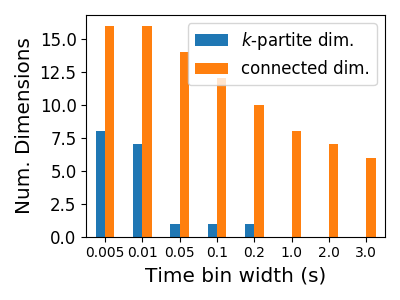
\includegraphics[width=\linewidth]{figures/Krebs_rectified_total_structure_dims.png}
      \label{fig:Krebs_rectified_total_structure_dims}
    \end{subfigure}
    \begin{subfigure}[h]{0.5\linewidth}
      \centering
      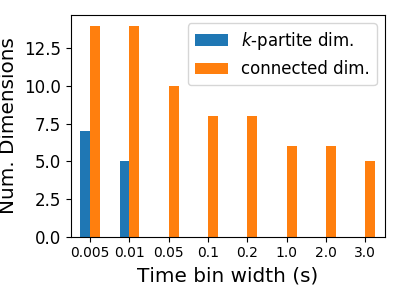
\includegraphics[width=\linewidth]{figures/Waksman_rectified_total_structure_dims.png}
      \label{fig:Waksman_rectified_total_structure_dims}
    \end{subfigure}
    \begin{subfigure}[h]{0.5\linewidth}
      \centering
      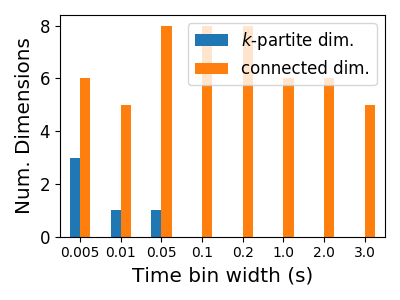
\includegraphics[width=\linewidth]{figures/Robbins_rectified_total_structure_dims.png}
      \label{fig:Robbins_rectified_total_structure_dims}
    \end{subfigure}
    \caption{The number of dimensions in the $k$-partite and connected structure in the correlation based networks beyond the structure captured by a sparse weighted configuration null network model (see section \ref{sec:sparse_weighted_configuration_model}), shown for different time bin widths. Note that the $k$-partite structure disappears for time bin width greater than $200$ms for all three subjects. The dimension of the connect structure reduces with increasing bin width for $2$ of the $3$ subjects (top row).}
    \label{fig:structure_dims}
  \end{figure}

  We chose the sparse weighted configuration model (see section \ref{sec:sparse_weighted_configuration_model}) as our null network model. This model matches the sparsity and the total weight of the original network but distributes the weight at random across the sparse network.

  We applied the spectral rejection method to our networks based on spike count correlations using different values for the time bin width. We observed that for smaller time bin widths, our data networks had both $k$-partite structure, and community structure. As the width of the time bin increased, we found that the $k$-partite structure disappeared from our data networks, and the dimension of the community strcuture reduced in two of the three mice from which we had data (see figure \ref{fig:structure_dims}).

  \subsection{Detecting communities in correlation based networks}

  \begin{figure}
    \begin{subfigure}[h]{0.5\linewidth}
      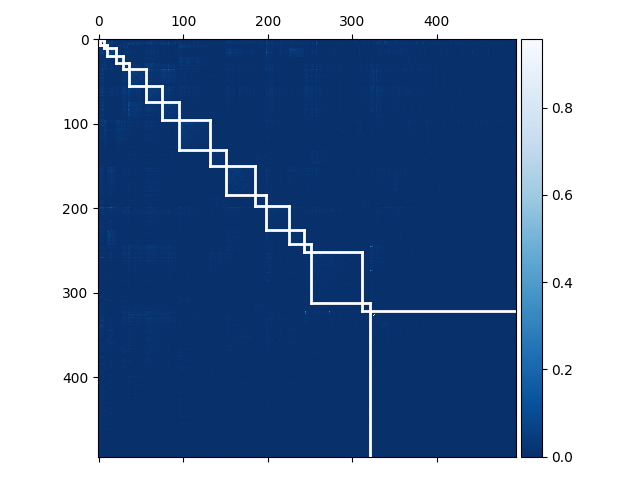
\includegraphics[width=\linewidth]{figures/Krebs_0p005_rectified_cons_cluster_map.png}
      \caption{5ms}
      \label{fig:consensus_cluster_5ms}
    \end{subfigure}
    \begin{subfigure}[h]{0.5\linewidth}
      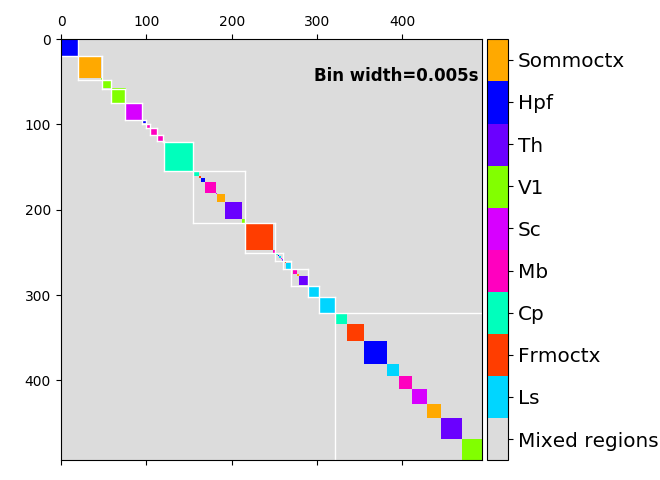
\includegraphics[width=\linewidth]{figures/Krebs_0p005_regional_cluster_map.png}
      \caption{5ms}
      \label{fig:regional_cluster_map_5ms}
    \end{subfigure}
    \begin{subfigure}[h]{0.5\linewidth}
      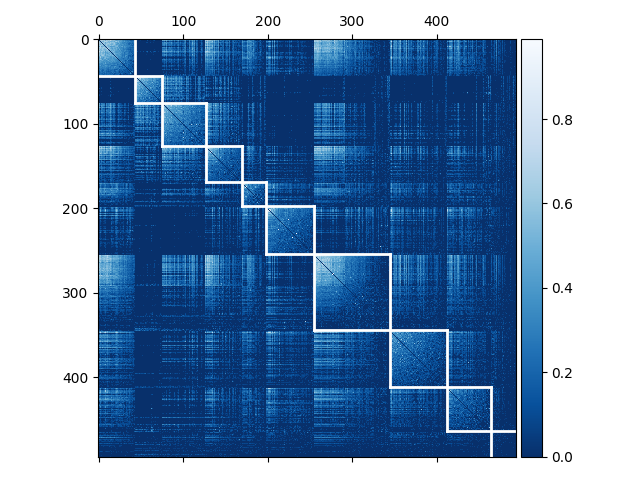
\includegraphics[width=\linewidth]{figures/Krebs_1p0_rectified_cons_cluster_map.png}
      \caption{1s}
      \label{fig:consensus_cluster_1s}
    \end{subfigure}
    \begin{subfigure}[h]{0.5\linewidth}
      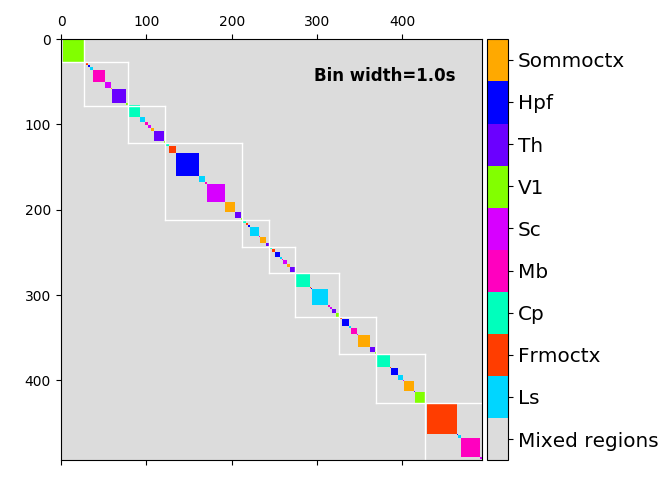
\includegraphics[width=\linewidth]{figures/Krebs_1p0_regional_cluster_map.png}
      \caption{1s}
      \label{fig:regional_cluster_map_1s}
    \end{subfigure}
    \caption{(a) and (c) Correlation matrices with detected communities indicated by white lines. Each off main diagonal entry in the matrix represents a pair of neurons. Those entries within a white square indicate that both of neurons are in the same community as detected by our community detection procedure. Matrices shown are for $5$ms and $1$s time bin widths respectively. (b) and (d) Matrices showing the anatomical distribution of pairs along with their community membership. Entries where both cells are in the same reigon are given a colour indicated on the colour bar. Entries where cells are in different regions are given the grey colour also indicated on the colour bar.}
    \label{fig:consensus_clusterings_with_regions}
  \end{figure}

  We applied the community detection procedure described in section \ref{sec:community_detection} to our signal networks for our various time bin widths. As might be expected from the results described above in section \ref{sec:dims_result}, we detected a greater number of smaller communities at shorter time bin widths, and a smaller number of larger communities for longer time bin widths (see figure \ref{fig:consensus_clusterings_with_regions}).

  We also noticed that at short time bin widths the communities detected tended to be dominated by cells from one region. Whereas communities existing in networks created using wider time bin widths tended to contain cells from many different brain regions. More on this in the next section.

% TODO: Need to expand the section in Methods on Community Detection.

  \subsection{Functional communities resemble anatomical division at short timescales}
  In order to quantify the similarity of the communities detected to the anatomical division of the cells. We treated both the anatomical division and the communities as clusterings of these cells. We then used measures for quantifying the difference or similarity between clusterings to quantify the difference or similarity between the detected communities and the anatomical division. Details of these measures can be found in section \ref{sec:clustering_comparison} or in \cite{vinh}.

  We used two different types of measures for clustering comparison; information based measures (see section \ref{sec:information_similarity_measures}) and pair counting based measures (see section \ref{sec:adjusted_rand_index}). We include one example of each in figure \ref{fig:distance_measures}.

  The variation of information is the information based measure included in figure \ref{fig:variation_of_information_rectified_total}. This measure forms a metric on the space of clusterings. The larger the value for the variation of information, the more different the clusterings.

  The adjusted Rand index is the pair counting based measure included in figure \ref{fig:adjusted_rand_index_rectified_total}. In contrast with the variation of information, the adjusted Rand index is a normalised similarity measure. The adjusted Rand index takes value 1 when the clusterings are identical, and takes value 0 when the clusterings are no more similar than chance.

  \begin{figure}[h]
    \begin{subfigure}[h]{0.5\linewidth}
      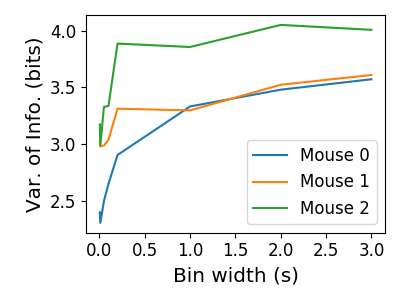
\includegraphics[width=\linewidth]{figures/variation_of_information_rectified_total.png}
      \caption{variation of information}
      \label{fig:variation_of_information_rectified_total}
    \end{subfigure}
    \begin{subfigure}[h]{0.5\linewidth}
      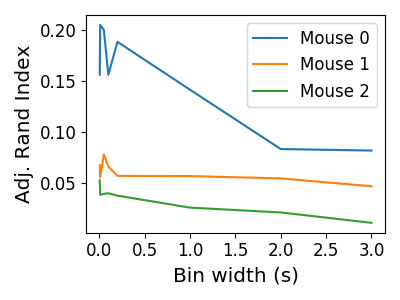
\includegraphics[width=\linewidth]{figures/adjusted_rand_index_rectified_total.png}
      \caption{Adjusted Rand index}
      \label{fig:adjusted_rand_index_rectified_total}
    \end{subfigure}
    \caption{distance measures between clusterings}
    \label{fig:distance_measures}
  \end{figure}

  Both measures indicated that the detected communities and the anatomical division of the cells were more similar at when we used shorter time bins widths (see figure \ref{fig:distance_measures}). This indicates that correlated behaviour in neuronal ensembles is more restricted to individual brain regions at short timescales (<$250$ms), and spreads out across brain regions at longer time scales.

  \subsection{Conditional correlations \& signal correlations}
  In light of Stringer et al (2019) showing that spontaneous behaviours can drive activity in neuronal ensembles across the visual cortex and midbrain\cite{stringer}, we decided to control for the mouse's behaviour when performing our analyses. My second supervisor, Dr Michael Ashby, suggested that our community detection process may be detecting communities across multiple brain regions at longer time scales due to aggregating neuronal activity driven by several spontaneous behaviours occuring during the time interval covered by a given time bin. A time bin of $1$s, for example, could contain a spike count where those spikes were driven by different spontaneous behaviours. We aimed to investigate this possibility by applying our community detection analysis to conditional correlation measures.

  We used the top $500$ principal components of a video of the mouse's face as a measure of the mouse's behaviour (see section \ref{sec:video_recordings}). We modelled the spike counts as a linear combination of the principal components using linear regression with ElasticNet regularisation (see section \ref{sec:conditioning_on_behavioural_data}). Using this model, we quantified the expected spike count given the mouse's behaviour $E[X|Z_1, \dots ,Z_{500}]$.

  \begin{figure}[h]
    \begin{subfigure}[h]{0.5\linewidth}
      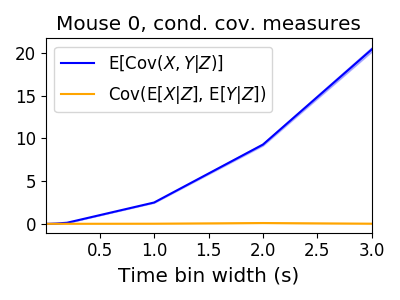
\includegraphics[width=\linewidth]{figures/Krebs_cond_cov_comparison.png}
      \label{fig:Krebs_cond_cov_comparison}
    \end{subfigure}
    \begin{subfigure}[h]{0.5\linewidth}
      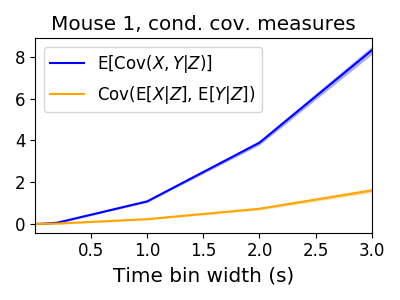
\includegraphics[width=\linewidth]{figures/Waksman_cond_cov_comparison.png}
      \label{fig:Waksman_cond_cov_comparison}
    \end{subfigure}
    \begin{subfigure}[h]{0.5\linewidth}
      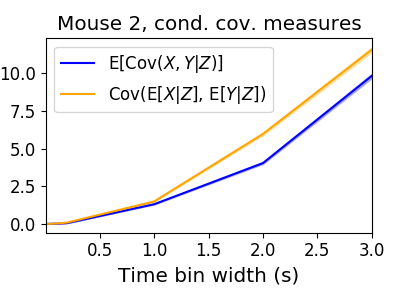
\includegraphics[width=\linewidth]{figures/Robbins_cond_cov_comparison.png}
      \label{fig:Robbins_cond_cov_comparison}
    \end{subfigure}
    \caption{Comparing the components of the spike count covariance across different values for the time bin width. We observed a consistent increase in $E[\cov (X,Y|Z)]$ as the time bin width increased. But we saw different trends for $\cov (E[X|Z], E[Y|Z])$ for each mouse.}
    \label{fig:conditional_covariance_comparison}
  \end{figure}

  We used these expected values to measure $\cov (E[X|Z], E[Y|Z])$, and we used that value, the covariance $\cov (X,Y)$, and the \textit{law of total covariance} (see section \ref{sec:conditional_covariance}) to measure $E[\cov (X,Y|Z)]$. Here $X$ and $Y$ represent spike counts from individual cells, and $Z$ is shorthand for the $500$ principal components mentioned above. The two components of the covariance, $\cov (E[X|Z], E[Y|Z])$ and $E[\cov (X,Y|Z)]$, represent a `signal covariance' and expected value of a `spike count covariance' respectively, analagous to the signal correlation and spike count correlation\cite{cohen2}.

  We examined the means of these components for different values of the time bin width (see figure \ref{fig:conditional_covariance_comparison}). We observed a consistent increase in $E[\cov (X,Y|Z)]$ as the time bin width increased. But we saw different trends for $\cov (E[X|Z], E[Y|Z])$ for each mouse.

  Using $\cov (E[X|Z], E[Y|Z])$ we measured the signal correlation, and using $E[\cov (X,Y|Z)]$ we measured the event conditional correlation (see section \ref{sec:cond_corr} for more details). We saw a consistent increase in $\rho_{X,Y|Z}$ as the time bin width increased, this corresponds to the result for $E[\cov(X,Y|Z)]$. We observed different trends for $\rho_{\text{signal}}$ for each mouse, this corresponds to the result for $\cov(E[X|Z],E[Y|Z])$.

  \begin{figure}[h]
    \begin{subfigure}[h]{0.5\linewidth}
      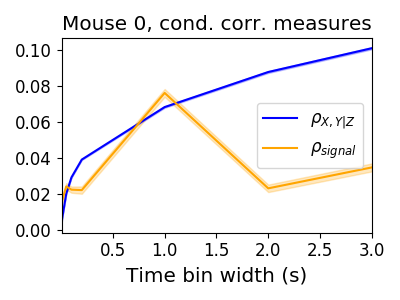
\includegraphics[width=\linewidth]{figures/Krebs_cond_corr_comparison.png}
      \label{fig:Krebs_cond_corr_comparison}
    \end{subfigure}
    \begin{subfigure}[h]{0.5\linewidth}
      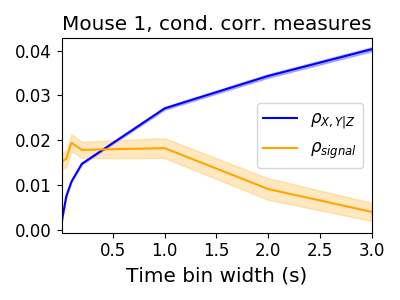
\includegraphics[width=\linewidth]{figures/Waksman_cond_corr_comparison.png}
      \label{fig:Waksman_cond_corr_comparison}
    \end{subfigure}
    \begin{subfigure}[h]{0.5\linewidth}
      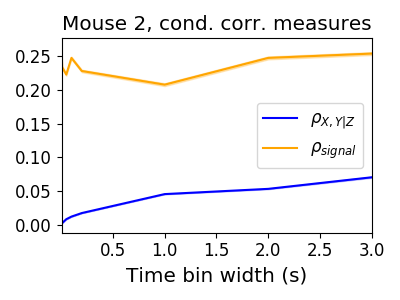
\includegraphics[width=\linewidth]{figures/Robbins_cond_corr_comparison.png}
      \label{fig:Robbins_cond_corr_comparison}
    \end{subfigure}
    \caption{Comparing the components of the total spike count covariance across different values for the time bin width. }
    \label{fig:conditional_correlation_comparison}
  \end{figure}

  We applied our network noise rejection and community detection process to networks based on the spike count correlations $\rho_{X,Y|Z}$ and the signal correlations $\rho_{\text{signal}}$. We noted that the community detection on $\rho_{X,Y|Z}$ behaved similarly to the community detection on the total spike count correlation. We can see this  in figures \ref{fig:short_time_conditional_rectified_regional_clusters} and \ref{fig:long_time_conditional_rectified_regional_clusters}. At very short time bin widths, we detect more communities, and those communities often contain cells from one brain region only. At longer time bin widths, we detect fewer communities, and those communities tend to contain cells from multiple brain regions. When we examine the distance between (or similarity between) the anatomical division of the cells, and the detected communities we notice that the two clusterings are more similar at shorter time bin widths (see figure \ref{fig:conditional_clustering_distance_measures}).

  \begin{figure}[h]
    \begin{subfigure}[h]{0.5\linewidth}
      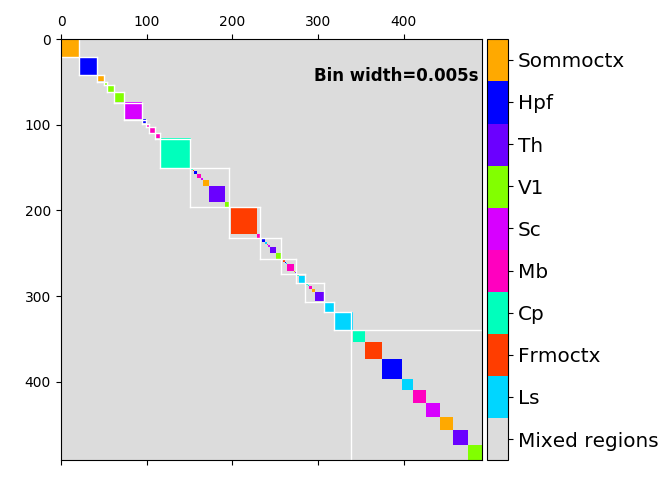
\includegraphics[width=\linewidth]{figures/Krebs_0p005_conditional_rectified_regional_cluster_map.png}
      \caption{$\rho_{X,Y|Z}$}
      \label{fig:short_time_conditional_rectified_regional_clusters}
    \end{subfigure}
    \begin{subfigure}[h]{0.5\linewidth}
      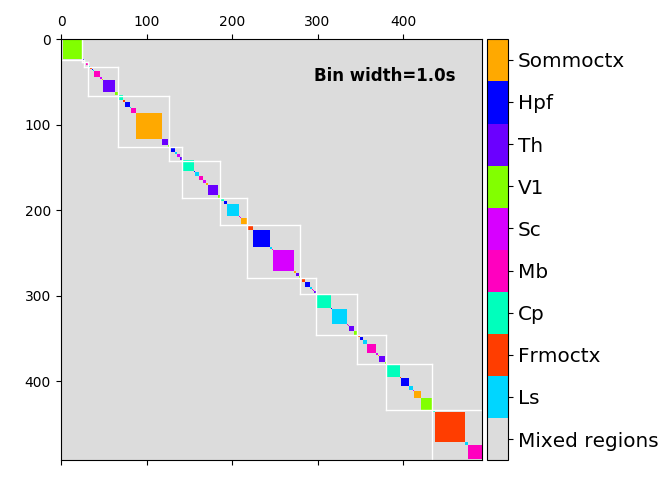
\includegraphics[width=\linewidth]{figures/Krebs_1p0_conditional_rectified_regional_cluster_map.png}
      \caption{$\rho_{X,Y|Z}$}
      \label{fig:long_time_conditional_rectified_regional_clusters}
    \end{subfigure}
    \begin{subfigure}[h]{0.5\linewidth}
      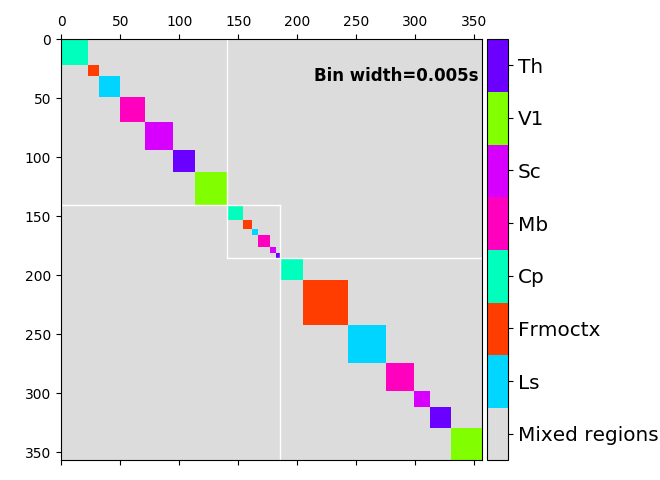
\includegraphics[width=\linewidth]{figures/Krebs_0p005_signal_rectified_regional_cluster_map.png}
      \caption{$\rho_{\text{signal}}$}
      \label{fig:short_time_signal_rectified_regional_clusters}
    \end{subfigure}
    \begin{subfigure}[h]{0.5\linewidth}
      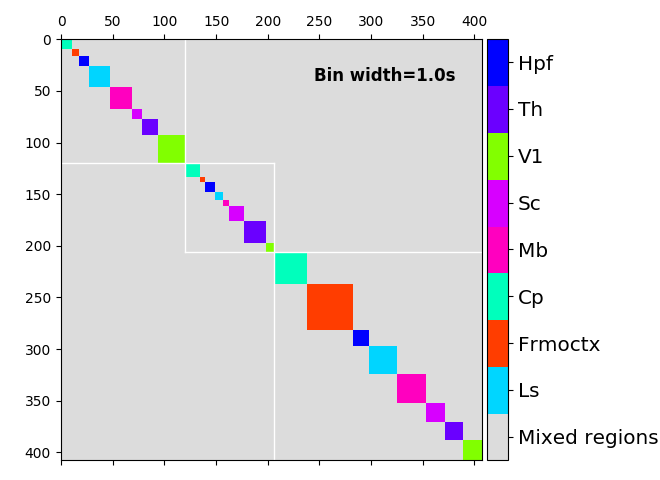
\includegraphics[width=\linewidth]{figures/Krebs_1p0_signal_rectified_regional_cluster_map.png}
      \caption{$\rho_{\text{signal}}$}
      \label{fig:long_time_signal_rectified_regional_clusters}
    \end{subfigure}
    \caption{Matrices showing the regional membership of pairs by colour, and the communities in which those pairs lie. (a-b) Detected communities and regional membership matrix for network based on rectified spike count correlation $\rho_{X,Y|Z}$, using time bin widths of $0.005$s and $1$s respectively. (c-d) Detected communities and regional membership matrix for network based on rectified signal correlation $\rho_{\text{signal}}$, using time bin widths of $0.005$s and $1$s respectively.}
    \label{fig:rectified_signal_regional_clusters}
  \end{figure}

  When we applied the network noise rejection and community detection process to the networks based on the signal correlations $\rho_{\text{signal}}$ we found the number of communities we detected reduced with increasing time bin width. But the number of communities detected was less than that for the total correalations or the spike count correlations. The communities detected always tended to contain cells from multiple regions at both short and long timescales (see figures \ref{fig:short_time_signal_rectified_regional_clusters} and \ref{fig:long_time_signal_rectified_regional_clusters}). The communities detected bore very little relation to the anatomical division of the cells. The adjusted Rand index between the community clustering and the anatomical `clustering' is close to zero for every time bin width (see figure \ref{fig:adjusted_rand_index_rectified_signal}). This indicates that the similarity between the clusterings is close to chance. We did observe a slight downward trend in the variation of information with increasing bin width (see figure \ref{fig:variation_of_information_rectified_signal}), but this is more likely due to a decrease in the number of communities detected rather than any relationship with anatomy.

  \begin{figure}[h]
    \begin{subfigure}[h]{0.5\linewidth}
      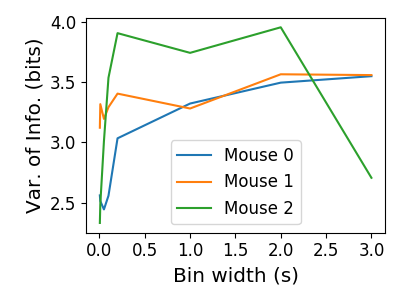
\includegraphics[width=\linewidth]{figures/variation_of_information_rectified_conditional.png}
      \caption{$\rho_{X,Y|Z}$ Variation of information.}
      \label{fig:variation_of_information_rectified_conditional}
    \end{subfigure}
    \begin{subfigure}[h]{0.5\linewidth}
      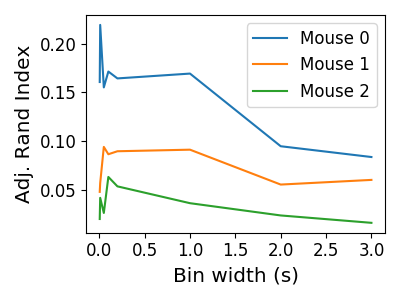
\includegraphics[width=\linewidth]{figures/adjusted_rand_index_rectified_conditional.png}
      \caption{$\rho_{X,Y|Z}$ Adjusted Rand Index.}
      \label{fig:adjusted_rand_index_rectified_conditional}
    \end{subfigure}
    \caption{Distance and similarity measures between the anatomical division of the neurons, and the communities detected in the network based on the spike count correlations $\rho_{X,Y|Z}$. (a) The variation of information is a `distance' measure between clusterings. The distance between the anatomical `clustering' and the community clustering increases as the time bin width increases. (b) The adjusted Rand index is a similarity measure between clusterings. The detected communities become less similar to the anatomical division of the cells as the time bin width increases.}
    \label{fig:conditional_clustering_distance_measures}
  \end{figure}

  \begin{figure}[h]
    \begin{subfigure}[h]{0.5\linewidth}
      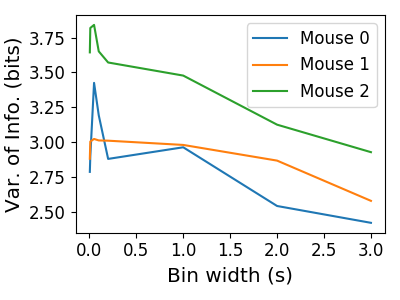
\includegraphics[width=\linewidth]{figures/variation_of_information_rectified_signal.png}
      \caption{$\rho_{\text{signal}}$ Variation of information.}
      \label{fig:variation_of_information_rectified_signal}
    \end{subfigure}
    \begin{subfigure}[h]{0.5\linewidth}
      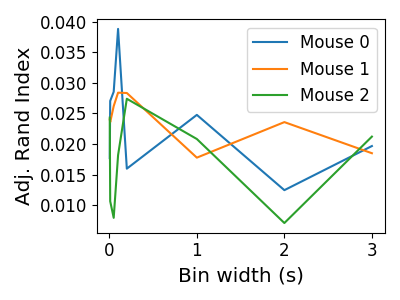
\includegraphics[width=\linewidth]{figures/adjusted_rand_index_rectified_signal.png}
      \caption{$\rho_{\text{signal}}$ Adjusted Rand Index.}
      \label{fig:adjusted_rand_index_rectified_signal}
    \end{subfigure}
    \caption{Distance and similarity measures between the anatomical division of the neurons, and the communities detected in the network based on the signal correlations $\rho_{\text{signal}}$. (a) The variation of information is a `distance' measure between clusterings. The distance between the anatomical `clustering' and the community clustering increases as the time bin width increases. (b) The adjusted Rand index is a similarity measure between clusterings. The detected communities become less similar to the anatomical division of the cells as the time bin width increases.}
    \label{fig:signal_clustering_distance_measures}
  \end{figure}

  % Figure 4: Conditional correlations
  % - Covariance matrices = conditional cov + signal cov
  % - Bar plot or similar comparing mean correlations for all three: total, conditional and signal.
  % - Corresponding plots for communities, one for conditional, one for signal, for both a short and long time bin
  % - VI measure vs time bins size for both types of correlation

  \subsection{Absolute correlations and negative rectified correlations}
  At the moment, the network noise rejection protocol can only be applied to weighted undirected graphs with non-negative weights. This meant that we had to rectify our correlated networks before applying the network noise rejection and community detection process. We wanted to investigate what would happen if instead of rectifying the correlations, we used the absolute value, or reversed the signs of the correlations and then rectified.

  When we used the absolute value of the correlations, we found very similar results to those shown above for the rectified correlations. The only exception being that we detected more communities. This could indicate that we detected both positively and negatively correlated communities, but we haven't done any further investigation so we cannot say for sure.

  When we used the sign reversed rectified correlated networks, we tended to find fewer communities and often found no signal network after applying network noise rejection. This indicates that there was not much structure in the negatively correlated networks beyond that captured by the sparse weighted configuration model.

\section{Discussion}
It is well established that the brain uses correlated behaviour in neuronal ensembles to represent the information taken in through the sensation\cite{cohen1, litwinkumar, decharms}. However, most studies that examine the nature of these correlations in-vivo, study an ensemble of cells from only one brain region\cite{cohen2}. Furthermore, recent results have shown that behaviour can drive correlated activity in multiple brain regions, including those not normally associated with motor control\cite{stringer}. In this study, we utilised one of the newly recorded large datasets containing electrophysiological recordings from multiple brain regions simultaneously. We investigated correlated behaviour in these different brain regions and we investigated correlated behaviour between neurons in different regions, during spontaneous behaviour.

A number of studies have found that the timescale of correlated behaviour induced by a stimulus can be modulated by the stimulus structure and behavioural context. For example, the spike train correlations between cells in weakly electric fish are modulated by the spatial extent of the stimulus\cite{litwinkumar}, and neurons in the marmoset primary auditory cortex modulate their spike timing (and therefore correlation) without modulating the firing rate in response to stimulus features\cite{decharms}. Furthermore, the width of the time bins over which spike counts are measured has been shown to have an effect on the magnitude of those correlations\cite{cohen2}. Despite this, very little research has been done comparing correlation measures from the same dataset at different timescales. We investigated this by varying the time bin width used to bin spike times into spike counts from as short as $5$ms up to $3$s.

In order to further investigate the effect of these correlations at different timescales, we regarded our neuronal ensemble as a weighted undirected graph, where each neuron is represented by a node, and the weight on each edge is the correlation between the neurons connected by that edge. We then applied a novel clustering method from network science\cite{humphries} to indentify communities in these networks. These networks, and the community detection process, were completely agnostic of anatomical division of the cells in our ensemble. When we compared the detected communities with the anatomical division of the cells using distance and similarity measures for clusterings, we found that the detected communities were more similar to the anatomical division and shorter timescales. That is, when we used a wider time bin to count spikes, and computed pairwise correlations with these spike counts, the correlated communities tended to exist within anatomical regions at shorter timescales, and tended to span anatomical regions at longer timescales. This could reflect localised functional correlations at short time scales rippling outwards across brain regions at longer timescales.

We acknowledged that the cross region correlated communities that we detected at longer time scales could be due to collating activity driven by various spontaneous activities. In order to account for this, we modelled the spike counts as a linear function of the top $500$ principal components of a video of the mouse's face filmed simultaneously with the electrophysiological readings. We did applied our network noise rejection and community detection process to the weighted undirected networks formed by the spike count correlations and the signal correlations that we calculated using our model. For the spike count correlation networks, we found much the same results as for the total correlations as described above. For the signal correlations, the communities detected in these networks bore little relation to the anatomical division of the cells.

There is a lot of room for further investigation based on this research. For a start, the data that we used here were collected from nine different regions in the mouse brain, but none of these regions were part of the somatosensory cortex. Given that a mouse experiences so much of its environment through its sense of smell, some data from this region would be interesting to investigate. On the same theme, the mice in the experiment from which the data were collected were headfixed and placed on a rotating ball, but were otherwise behaving spontaneously. Had these mice been exposed to a visual, aural, or olfactory stimulus, we could have examined the responses of the cells in the brain regions corresponding to vision, hearing, and olfaction, and compared these responses to the responses from the other brain regions. Furthermore, we could have investigated the interaction between the sets of responses.

Another space for further investigation is the community detection. The algorithm that we used here never detects overlapping communities. But functional communities could indeed have overlaps. Clustering methods that detect overlapping clusters do exist\cite{baadel}. Applying one of those algorithms could yield some interesting results. Also, the community detection algorithm that we used here cannot process graphs with negative weights, this forced us to separate positive and negative correlations before applying our network noise rejection and community detections process, or use the absolute value of our correlations. A community detection algorithm that can work on weighted undirected graphs with negative weights could yield some interesting results here.

\section{Data}

    The data that we used in this project were collected by Nick Steinmetz and his lab members\cite{stringer}.

    \subsection{Brain regions}
    Neuropixels probes were used to collect extracellular recordings \cite{jun} from three different mice. The mice were awake, headfixed, and engaging in spontaneous behaviour. The mice were of different sexes and different ages. One mouse was `wild-type', the others were mutants. Details as follows:
    \begin{enumerate}
        \item male, wild type, P73. % Robbins
        \item female, TetO-GCaMP6s, Camk2a-tTa, P113 % Waksman
        \item male, Ai32, Pvalb-Cre, P99 % Krebs
    \end{enumerate}

    Eight probes were used to collect readings from 2296, 2668, and 1462 cells respectively. Data were collected from nine brain regions in each mouse:
    \begin{itemize}
        \item Caudate Putamen (CP)
        \item Frontal Motor Cortex (Frmoctx)
        \item Hippocampal formation (Hpf)
        \item Lateral Septum (Ls)
        \item Midbrain (Mb)
        \item Superior Colliculus (Sc)
        \item Somatomotor cortex (Sommoctx)
        \item Thalamus (Th)
        \item Primary visual cortex (V1)
    \end{itemize}
    Readings were continuous and lasted for about 1 hour \cite{stringer}. Locations of each of the probes can be seen in figure \ref{fig:probe_locations}.

    \begin{figure}[h]
        \centering
        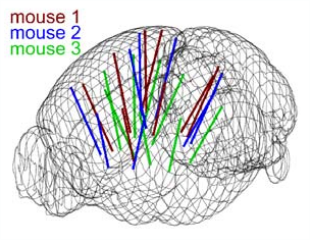
\includegraphics[width=5cm,height=3.75cm]{figures/probe_locations_stringer.png}
        \caption{\textbf{Probe Locations:} The locations of the probes in each of the three mouse brains\cite{stringer}.}
        \label{fig:probe_locations}
    \end{figure}

    \subsection{Video recordings}\label{sec:video_recordings}
    Video recordings of the mouse's face were taken during the spontaneous behaviour. We had access to the top $500$ principle components and top $500$ eigenvectors of the processed videos. The frequency of recording was slightly less than $40$Hz. Each frame contained $327 \times 561$ pixels. These principal components were used as behavioural data. We controlled for these components when taking measurements conditioned on behaviour.

\section{Methods}
    \subsection{Binning data}
    We transoformed the spike timing data into binned spike count data by dividing the experimental period into time bins and counting the spikes fired by each cell within the time period covered by each of those bins. The data were divided into time bins of various widths ranging from $0.01$s to $4$s.

    If the total length of the recording period was not an integer multiple of the time bin width, we cut off the remaining time at the end of the recording period. This period was at most $3.99$s. This is far less than the total recording time of around $1$ hour. So, this detail would not affect our results.

    \subsection{Correlation coefficients}
    We calculated Pearson's correlation coefficient for pairs of spike counts from pairs of neurons. For jointly distributed random variables $X$ and $Y$, Pearson's correlation coefficient is defined as:
    \begin{align}\label{eq:dist_pearsons_corr}
        \rho_{XY} =& \frac{\cov(X,Y)}{\sigma_X \sigma_Y} \\
                  =& \frac{E[(X - \mu_X)(Y - \mu_Y)]}{\sigma_X \sigma_Y}
    \end{align}
    where $E$ denotes the expected value, $\mu$ denotes the mean, and $\sigma$ denotes the standard deviation. The correlation coefficient is a normalised measure of the covariance. It can take values between $1$ (completely correlated) and $-1$ (completely anti-correlated). Two independent variables will have a correlation coefficient of $0$. But, having $0$ correlation does not imply independence.

    If we do not know the means and standard deviations required for equation \ref{eq:dist_pearsons_corr}, but we have samples from $X$ and $Y$, Pearson's sample correlation coefficient is defined as:
    \begin{align}
        r_{XY} = \frac{\sum_{i=1}^n (x_i - \bar{x})(y_i - \bar{y})}{\sqrt{\sum_{i=1}^n (x_i - \bar{x})^2}\sqrt{\sum_{i=1}^n (y_i - \bar{y})^2}}
    \end{align}
    where $\lbrace (x_i, y_i) \rbrace$ for $i \in \lbrace 1, \dots, n \rbrace$ are the paired samples from $X$ and $Y$, and $\bar{x} = \frac{1}{n}\sum_{i=1}^n x_i$, and $\bar{y} = \frac{1}{n}\sum_{i=1}^n y_i$ are the sample means.

    In practice we used the python function \texttt{scipy.stats.pearsonr} to calculate the correlation coefficients.

        \subsubsection{Spike Count Correlation, $r_{SC}$}\label{sec:spike_count_correlation}
        The spike count correlation ($r_{SC}$) of two cells is the correlation between the spike counts of those cells in response to a given stimulus condition. In this study, there was only one stimulus condition, that of no stimulus. The subjects engaged in spontaneous behaviour during recording.

        \subsubsection{Shuffled spike count correlations}\label{sec:shuffled_correlations}
        We measured the shuffled spike count correlations between two neurons by randomly permuting one of the neuron's spike counts and measuring the spike count correlations. These shuffled correlations were useful when measuring the effect of time bin width on correlations, and when deciding which correlations should be preserved when creating correlation networks (see section \ref{sec:sparsifying_data_networks}).

        \subsubsection{Separating Correlations \& Anti-correlations}\label{sec:corr_anti_corr}
        In order to compare the effect of bin width on measures of negative $r_{SC}$ (anti-correlation) and positive $r_{SC}$ separately, we had to separate correlated and anti-correlated pairs. To do this, we simply measured the mean $r_{SC}$, taking the mean across all the bin widths. If this quantity was positive or zero we regarded the pair as positively correlated. If this quantity was negative we regarded the pair as anti-correlated.

    \subsection{Conditioning on behavioural data}\label{sec:conditioning_on_behavioural_data}
    Our behavioural data consisted of the top $500$ principal components (PCs) of a processed video recording of the mouse's face (see section \ref{sec:video_recordings}). Denoting the spike count of a given cell by $X$, and the PCs by $Z_1,\dots,Z_{500}$, we wanted to model $X$ as a function of $Z_1,\dots,Z_{500}$ in order to estimate
    \begin{align}
      E[X|Z_1,\dots,Z_{500}] &= \int_{x \in X} x P(X=x | Z_1,\dots,Z_{500}) dx \\
        &= \int_{x \in X} x \frac{P(X=x, Z_1,\dots,Z_{500})}{P(Z_1,\dots,Z_{500})} dx
    \end{align}
    Given the $500$ components, a na\"{i}ve estimation of $P(Z_1,\dots,Z_{500})$ or $P(X, Z_1,\dots,Z_{500})$ by histogramming was impossible. Therefore we modelled $X$ as a linear combination of the PCs.

        \subsubsection{Linear regression}
        We modelled the spike count of a given cell, $X$, as a linear combination of the PCs of the video of the mouse's face, $\mathbf{Z} = Z_1,\dots,Z_{500}$. We tried three different types of regularization
        \begin{itemize}
            \item $L1$ or `Lasso'
            \item $L2$ or `Ridge regression'
            \item `Elastic net' regularisation (a linear combination of both $L1$ and $L2$ regularisation penalities)
        \end{itemize}
        The elastic net regularisation performed the best, so we stuck with that.

        \subsubsection{Elastic net regularisation}
        Suppose we wish to model $n$ observations of a random variable $X$, $\mathbf{x} = (x_1, \cdots, x_n)$ using $n$ instances of $m$ predictors $\mathbf{Z} = (Z_1, \cdots, Z_m)$. The na\"{i}ve elastic net criterion is
        \begin{align}\label{eq:elastic_net}
            L(\lambda_1, \lambda_2, \boldsymbol{\beta}) = | \mathbf{x} - \mathbf{Z} \boldsymbol{\beta} |^2 + \lambda_2 |\boldsymbol{\beta}|_2 + \lambda_1 |\boldsymbol{\beta}|_1
        \end{align}
        where
        \begin{align}
          |\boldsymbol{\beta}|_2 &= \sum_{j=1}^m \beta_j^2 \\
          |\boldsymbol{\beta}|_1 &= \sum_{j=1}^m |\beta_j|
        \end{align}
        The na\"{i}ve elastic net estimator $\hat{\boldsymbol{\beta}}$ is the minimiser of the system of equations \ref{eq:elastic_net} \cite{zou}
        \begin{align}
          \hat{\boldsymbol{\beta}} = \arg \min_{\boldsymbol{\beta}} L(\lambda_1, \lambda_2, \boldsymbol{\beta})
        \end{align}
        We implemented the model using the \texttt{ElasticNetCV} method of Python's \\ \texttt{sklearn.linear\_models} package.

        As well as using the PCs, we also tried fitting the models using the raw video data reconstructed from the PCs and eigenvectors. These models performed worse than those using the PCs. We expected this because each representation contains the same amount of information, but the raw video representation spreads this information across many more components. This requires more parameter fitting, but given the same information.

        \subsubsection{Conditional covariance}\label{sec:conditional_covariance}
        We calculated the expected value of the conditional covariance using the law of total covariance.
        \begin{align}\label{eq:law_of_total_covariance}
            \cov (X,Y) = E[ \cov(X,Y|Z)] + \cov(E[X|Z], E[Y|Z])
        \end{align}
        where these expected values are calculated with respect to the distribution of $Z$ as a random variable.

        The law of total covariance breaks the covariance into two components. The first component $E[\cov(X,Y|Z)]$ is the expected value, under the distribution of $Z$, of the conditional covariance $\cov(X,Y|Z)$. This covariance could be interpreted as the unnormalised version of what Cohn et al. (2011) call the spike count correlation\cite{cohen2}, aka. the noise correlation. In particular, this is the covariance of the spike counts in response to repeated presentation of identical stimului.

        The second component is analogous to what Cohn et al. (2011) call the \textit{signal correlation}\cite{cohen2}. In particular, $\cov(E[X|Z], E[Y|Z])$ is the covariance between spike counts in response to different stimuli.

        Using our linear model, we calculated $E[X|Z_1,\dots, Z_{500}]$ for each cell $X$. Then we proceeded to calculate
        \begin{align}
            E[\cov(X,Y|Z_1,\dots, Z_{500})] = & \cov(X,Y) - \\
              & \cov(E[X|Z_1,\dots, Z_{500}], E[Y|Z_1,\dots, Z_{500}])
        \end{align}

        \subsubsection{Measures of conditional correlation}\label{sec:cond_corr}
        As a measure of expected correlation, we measured the `event conditional correlation' \cite{maugis}
        \begin{align}\label{eq:event_conditional_correlation}
            \rho_{XY|Z} = \frac{E[\cov(X,Y|Z)]}{\sqrt{E[\var(X|Z)]E[\var(Y|Z)]}}
        \end{align}
        Although this is not an actual correlation, it is an intuitive analogue to the correlation as a normalised version of the covariance.

        For comparison, we also measured the `signal correlation'
        \begin{align}\label{eq:signal_correlation}
            \rho_{\text{signal}} = \frac{\cov(E[X|Z], E[Y|Z])}{\sqrt{\var(E[X|Z])\var(E[Y|Z])}}
        \end{align}
        this is an actual correlation.

    \subsection{Information Theory}\label{sec:information_theory}
        \subsubsection{Entropy $H(X)$}
        The entropy of a random variable $X$, with outcomes $x_1, \dots, x_N$, and corresponding probabilities $p_1, \dots, p_N$ is defined as
        \begin{align}\label{entropy}
        H(X) = -\sum_{n=1}^N p_n \log _2 p_n
        \end{align}
        This quantity is also known as the information entropy or the `surprise'. It measures the amount of uncertainty in a random variable. For example, a variable with a probability of $1$ for one outcome, and $0$ for all other outcomes will have 0 bits entropy, because it contains no uncertainty. But a variable with a uniform distribution will have maximal entropy as it is the least predictable. This quantity is analogous to the entropy of a physical system \cite{shannon}. Note that any base may be used for the logarithm in equation \ref{entropy}, but using base $2$ means that the quantity will be measured in `bits'.

        The joint entropy of two jointly distributed random variables $X$ and $Y$, where $Y$ has outcomes $y_1, \dots, y_M$, is defined as
        \begin{align}\label{joint_entropy}
        H(X, Y) = -\sum_{n=1}^N \sum_{m=1}^M P(X=x_n, Y=y_m) \log _2 P(X=x_n, Y=y_m)
        \end{align}
        If $X$ and $Y$ are independent then $H(X,Y) = H(X) + H(Y)$. Otherwise $H(X,Y) < H(X) + H(Y)$. When $X$ and $Y$ and completely dependent $H(X,Y) = H(X) = H(Y)$.

        The conditional entropy of $Y$ conditioned on $X$ is defined as
        \begin{align}
        H(Y|X) = -\sum_{n=1}^N \sum_{m=1}^M P(X=x_n, Y=y_m) \log _2 \frac{P(X=x_n, Y=y_m)}{P(X=x_n)}
        \end{align}
        When $X$ and $Y$ are independent $H(Y|X) = H(Y)$. Intuitively, we learn nothing of $Y$ by knowing $X$, so $Y$ is equally uncertain whether we know $X$ or not. If $Y$ is totally dependent on $X$, then the fraction in the logarithm is $1$, which gives $H(Y|X) = 0$.

        These entropy measures are the basis of the mutual information measure.

        \subsubsection{Maximum entropy limit}\label{sec:entropy_limit}
        When spiking data is binned into spike counts there is an upper limit on the entropy of these data. The maximum entropy discrete distribution is the discrete uniform distribution. A random variable with this distribution will take values from some finite set with equal probabilities. Binned spike count data will take values between $0$ and some maximum observed spike count $n_{\max}$. A neuron with responses that maximises entropy will take these values with equal probability, i.e. if $i \in \lbrace 0, \dots, n_{\max} \rbrace$ then $P(X = i) = \frac{1}{n_{\max} + 1}$. The entropy of this neuron will be
        \begin{align*}
          H(X)  &= - \sum_{i=0}^{n_{\max}} P(X = i) \log _2 P(X=i) \\
                &= - \sum_{i=0}^{n_{\max}} \frac{1}{n_{\max} + 1} \log_2 \left( \frac{1}{n_{\max} + 1} \right) \\
                &= - \log_2 \left( \frac{1}{n_{\max} + 1} \right) \\
                &= \log_2 \left( n_{\max} + 1 \right)
        \end{align*}
        Therefore, the maximum entropy of the binned spike counts of a neuron is $\log _2 \left( n_{\max} + 1 \right)$. Of course, it would be very unusual for a neuron to fire in accordance with the discrete uniform distribution. Most measurements of entropy taken on binned spiking data will be much lower than the maximum. See figure \ref{fig:entropy_limit} to see the maximum entropy as a function of the maximum observed spike count.

        \begin{figure}[h]
          \centering
          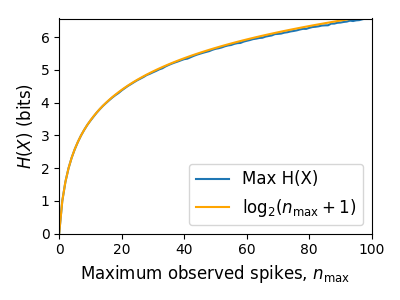
\includegraphics[width=0.5\textwidth]{figures/entropy_limit.png}
          \caption{\textbf{Entropy Limit:} The upper limit on entropy of binned spike count data as a function of the maximum observed spike count. The orange line is the analytical maximum. The blue line is the entropy of samples with $N=1000$ data points taken from the discrete uniform distribution.}
          \label{fig:entropy_limit}
        \end{figure}

        \subsubsection{Mutual Information $I(X;Y)$}
        The mutual information can be defined mathematically in a number of ways, all of which are equivalent. These definitions illustrate the different ways of interpreting the mutual information.

        For two jointly distributed random variables $X$ and $Y$, the mutual information $I(X;Y)$ is defined as
        \begin{align}\label{eq:mutual_info_intuitive}
            I(X;Y)  =& H(Y) - H(Y|X) \\
                    =& H(X) - H(X|Y)
        \end{align}
        Equation \ref{eq:mutual_info_intuitive} fits with the following intuition: The mutual information between $X$ and $Y$ is the reduction in uncertainty about $X$ gained by knowing $Y$, or vice versa. We could also say the mutual information is the amount of information gained about $X$ by knowing $Y$, or vice versa.

        Another useful entropy based definition for the mutual information is
        \begin{align}\label{eq:mutual_info_useful}
            I(X;Y)  =& H(X) + H(Y) - H(X,Y)
        \end{align}
        This definition is useful because it does not require the calculation of conditional probabilities.

        The mutual information can also be defined in terms of marginal, joint, and conditional distributions. For example,
        \begin{align}\label{eq:mutual_info_log}
            I(X;Y)  =& -\sum_{n=1}^N \sum_{m=1}^M P(X=x_n, Y=y_m) \log _2 \frac{P(X=x_n, Y=y_m)}{P(X=x_n) P(Y=y_m)}
        \end{align}
        Notice that this can be rewritten as a Kullback–Leibler divergence.
        \begin{align}
            I(X;Y)  =& D_{KL}(P(X,Y)|| P(X)P(Y))
        \end{align}
        So, we can also think of the mutual information as a measure of the difference between the joint distribution of $X$ and $Y$, and the product of their marginal distributions. Since the product of the marginal distributions is the joint distribution for independent variables, we can think of the mutual information as a measure of the variables' dependence on one another.

        The minimum value that $I(X;Y)$ can take is $0$. This occurs when the random variables $X$ and $Y$ are independent. Then we have $H(X|Y) = H(X)$, and $H(Y|X) = H(Y)$, which according to equation \ref{eq:mutual_info_intuitive}, gives $I(X;Y) = 0$. We also have that $H(X,Y) = H(X) + H(Y)$ in this case, which according equation \ref{eq:mutual_info_useful}, gives $I(X;Y) = 0$. Finally, we also have $P(X,Y) = P(X)P(Y)$, which leaves us with $1$ in the argument for the logarithm in equation \ref{eq:mutual_info_log}, which again gives $I(X;Y) = 0$.

        The mutual information reaches its maximum value when one of the variables $X$ and $Y$ is completely determined by knowing the value of the other. In that case $I(X;Y) = \min \lbrace H(X), H(Y) \rbrace$.

        \subsubsection{Variation of Information $VI(X,Y)$}\label{sec:variation_of_information}
        The variation of information is another information theoretical quantity based on the mutual information. It is defined as
        \begin{align}\label{eq:variation_of_information}
            VI(X;Y) = H(X) + H(Y) - 2 I(X;Y)
        \end{align}
        We can rewrite this as the summation of two positive quantities
        \begin{align}
            VI(X;Y) = \left[ H(X) - I(X;Y) \right] + \left[ H(Y) - I(X;Y) \right]
        \end{align}
        In English, the variation of information is the summation of the uncertainty in the random variables $X$ and $Y$ excluding the uncertainty shared by those variables.

        This measure will become more relevant when we go on to talk about clusterings because $VI(X;Y)$ forms a metric on the space of clusterings.

        \subsubsection{Measuring entropies \& mutual information}
        In practice, we measured the mutual information between spike counts using Python and the python package \texttt{pyitlib}. We used the PT-bias correction technique to estimate the bias of our measurements when measuring the mutual information between the spike counts of two cells \cite{treves}.

        When measuring the mutual information between clusterings we used Python, but we used the \texttt{mutual\_info\_score}, \texttt{adjusted\_mutual\_info\_score}, and \\ \texttt{normalized\_mutual\_info\_score} functions from the \texttt{sklearn.metrics} part of the \texttt{sklearn} package.

    \subsection{Network analysis}
        \subsubsection{Correlation networks}
        In order to analyse functional networks created by the neurons in our ensemble, we measured the spike count correlation between each pair of neurons. These measurements induced an undirected weighted graph/network between the neurons. The weight of each connection was equal to the spike count correlation between each pair of neurons.

        We followed the same procedure for spike count correlations \ref{sec:spike_count_correlation}, conditional correlations, and signal correlations \ref{sec:cond_corr}.

        \subsubsection{Rectified correlations}
        At the time of writing, the community detection method outlined in \cite{humphries} could only be applied to networks with positively weighted connections. But many neuron pairs were negatively correlated. To apply the community detection method, we \textit{rectified} the network, by setting all the negative weights to zero.

        We also looked for structure in the network created by negative correlations by reversing the signs of the correlations, and rectifying these correlations before applying our network analysis.

        Finally, we used the absolute value of the correlations as the weights for the graph/network. By doing this, we hoped to identify both correlated and anti-correlated functional communities of neurons.

        \subsubsection{Sparsifying data networks}\label{sec:sparsifying_data_networks}
        When creating our correlation networks, we wanted to exclude any correlations that could be judged to exist `by chance'. To do this, we measured the $5$th and $95$th percentile of the shuffled correlations (see section \ref{sec:shuffled_correlations}) for the given mouse and time bin width. We then set all the data correlations between these two values to $0$. This excluded any `chance' correlations from our network, and created a sparser network. This allowed us to make use of the `sparse weighted configuration model' as described in section \ref{sec:sparse_weighted_configuration_model}.

        \subsubsection{Communities}
        Given some network represented by an adjacency matrix $\mathbf{A}$, a community within that network is defined as a collection of nodes where the number of connections within these nodes is higher than the expected number of connections between these nodes. In order to quantify the `expected' number of connections, we need a model of expected networks. This is analogous to a `null model' in traditional hypothesis testing. We test the hypothesis that our data network departs from the null network model to a statistically significant degree. For undirected unweighted networks, the canonical model of a null network is the configuration model \cite{fosdick}. Since we are working with weighted sparse networks, we used more suitable null models, described below.

        \subsubsection{Weighted configuration model}\label{sec:weight_configuration_model}
        The \textit{weighted configuration model} is a canonical null network model for weighted networks. Given some data network, the weighted configuration model null network will preserve the degree sequence and weight sequence of each node in the data network. But the edges will be distributed randomly \cite{fosdick}. Any structure in the data network beyond its degree sequence and weight sequence will not be captured in the weighted configuration model. So, this model can be used in testing the hypothesis that this extra structure exists.

        \subsubsection{Sparse weighted configuration model}\label{sec:sparse_weighted_configuration_model}
        The \textit{sparse weighted configuration model} is another null network model. Similar in nature to the weighted configuration model (see section \ref{sec:weight_configuration_model}), but the sparsity of the data network is preserved in the null network. This is achieved by sampling from a probability distribution for the creation or non-creation of each possible connection, then distributing the weight of the data network randomly in this sparse network \cite{humphries}. This is the null network that we used when searching for additional strcuture in our data networks.

        \subsubsection{Spectral rejection}\label{sec:spectral_rejection}
        We made use of the spectral rejection algorithm as outlined in \cite{humphries}. The spectral rejection algorithm is a method for finding structure in a network not captured by a supposed null model, if such structure exists.

        To describe the method, we denote our data network matrix $\mathbf{W}$, we denote the expected network of our null network model as $\left\langle \mathbf{P} \right\rangle$. Then the departure of our data network from the null network can be described by the matrix
        \begin{align}
          \mathbf{B} = \mathbf{W} - \left\langle \mathbf{P} \right\rangle
        \end{align}
        a common choice for $\left\langle \mathbf{P} \right\rangle$ in community detection is the `configuration model' \cite{fosdick, humphries2}. The matrix $\mathbf{B}$ is often called the configuration matrix, in this context we will use the term `deviation matrix' as it captures the deviation of $\mathbf{W}$ from the null model.

        To test for structure in the network represented by $\mathbf{W}$, we examine the eigenspectrum of $\mathbf{B}$ and compare it to the eigenspectrum of our null model. Firstly, note that since our data model doesn't allow self loops, and is not directed, the matrix representing the network will be symmetric and positive semi-definite, and will therefore be invertible with real eigenvalues. We selected a null model with the same characteristics.

        To find the eigenspectrum of the null model, we generated $N$ samples from our null model $P_1, \dots, P_N$, and we measured their deviation matrices $B_1, \dots, B_N$. We then calculated the eigenspectrum of each of those samples. We calculated the upper bound of the null model eigenspectrum by taking the mean of the largest eigenvalues of $B_1, \dots, B_N$. We calculated a lower bound on the null model eigenspectrum by taking the mean of the smallest eigenvalues of $B_1, \dots, B_N$.

        We then calculated the eigenspectrum of $\mathbf{B}$, our data network deviation matrix. If any of those eigenvalues lay outside of the upper or lower bounds of the null model eigenspectrum, this is evidence of additional structure not captured by the null model. If we chose the sparse weighted configuration model (see section \ref{sec:sparse_weighted_configuration_model}) as our null network model, then eigenvalues lying below the lower bound indicate $k$-partite structure in the network. For example, if one eigenvalue lay below the lower bound, this would indicate some bipartite structure in the data network. If any eigenvalues lay above the upper bound of the null model eigenspectrum, this is evidence of community structure in the data network. For example, one eigenvalue of $\mathbf{B}$ lying above the upper bound of the null model eigenspectrum indicates the presence of two communities in the network \cite{humphries2}.

        \subsubsection{Node rejection}\label{sec:node_rejection}
        If there are $d$ data eigenvalues lying outside of the null network eigenspectrum, the $d$ eigenvectors corresponding to these eigenvalues will form a vector space. If we project the nodes of our network into this vector space, by projecting either rows or colmns of the data matrix, we can see how strongly each node contributes to the vector space. Nodes that contribute strongly to the additional structure will project far away from the origin, nodes that do not contribute to the additional structure will project close to the origin. We want to use this information to discard those nodes that do not contribute.

        We can test whether a node projects \textit{far} away from the origin or \textit{close} to the origin using the eigenvalues and eigenvectors of $B_1, \dots, B_N$. The $j$th eigenvector and eigenvalue of $B_i$ gives a value for a null network's projection into the $j$th dimension of the additional structure vector space. The matrices $B_1, \dots, B_N$ give $N$ projections into that dimension. These projections are a distribution of the null networks' projections. If the data node's projection exceeds that of the null network projections this node is judged to project \textit{far} from the origin, and therefore contribute to the additional structure. Otherwise, the node is judged to project \textit{close} to the origin, and is therefore rejected \cite{humphries}.

        \subsubsection{Community detection}\label{sec:community_detection}
        Another application for this $d$ dimensional space is community detection. We first project all of the nodes into this $d$-dimensional space, then perform the clustering in this space. The clustering and community detection procedure is described in \cite{humphries2}.

        In practice, the procedure is carried out $n$ times (we chose $n=100$ times), this returns $n$ clusterings. We resolve these $n$ clusterings to one final clustering using \textit{consensus clustering}. We used the consensus clustering method that uses an explicit null model for the consensus matrix, as outlined in \cite{humphries}.

    \subsection{Clustering Comparison}\label{sec:clustering_comparison}
    A clustering $\mathcal{C}$ is a partition of a set $D$ into sets $C_1, C_2, \dots, C_K$, called clusters, that satisfy the following for all $k,l \in \lbrace 1,\dots,K \rbrace$:
    \begin{align}
        C_k \cap C_l &= \emptyset \\
        \bigcup_{k=1}^K C_k &= D
    \end{align}
    If we consider two clusterings, $\mathcal{C}$ with clusters $C_1, C_2, \dots, C_K$ and $\mathcal{C}^{\prime}$ with clusters \\ $C_1^{\prime}, C_2^{\prime}, \dots, C_K^{\prime}$. There are a number of measurements we can use to compare $\mathcal{C}$ and $\mathcal{C}^{\prime}$. In the following, the number of elements in $D$ is denoted by $n$, and the number of elements in cluster $C_k$ is $n_k$.

      \subsubsection{Adjusted Rand Index}\label{sec:adjusted_rand_index}
      The \textit{adjusted Rand Index} is a normalised similarity measure for clusterings based on pair counting.

      If we consider the clusterings $\mathcal{C}$ and $\mathcal{C}^{\prime}$, and denote
      \begin{itemize}
        \item the number of pairs in the same cluster in $\mathcal{C}$ and $\mathcal{C}^{\prime}$ by $N_{11}$
        \item the number of pairs in different clusters in $\mathcal{C}$ and $\mathcal{C}^{\prime}$ by $N_{00}$
        \item the number of pairs in the same cluster in $\mathcal{C}$ and different clusters in $\mathcal{C}^{\prime}$ by $N_{10}$
        \item the number of pairs in different clusters in $\mathcal{C}$ and the same cluster in $\mathcal{C}^{\prime}$ by $N_{01}$
      \end{itemize}
      then the \textit{Rand Index} is defined as
      \begin{align}
          RI = \frac{N_{11} + N_{00}}{N_{11} + N_{00} + N_{10} + N_{01}} = \frac{N_{11} + N_{00}}{\binom{n}{2}}
      \end{align}
      The Rand Index is $1$ when the clusterings are identical, and $0$ when the clusterings are completely different.

      The \textit{adjusted Rand Index} intends on correcting the Rand Index for chance matching pairs. This is defined as
      \begin{align}
          ARI = \frac{2\left( N_{00}N_{11} - N_{01}N_{10} \right)}{\left( N_{00} + N_{01} \right)\left( N_{01} + N_{11} \right) + \left( N_{00} + N_{10} \right)\left( N_{10} + N_{11} \right)}
      \end{align}
      The adjusted Rand Index is $1$ when the clusterings are identical, and $0$ when the Rand Index is equal to its expected value.

      \subsubsection{Clusterings as random variables}
      If we take any random element of $D$, the probability that this element is in cluster $C_k$ of clustering $\mathcal{C}$ is
      \begin{align}
          P(K=k) = \frac{n_k}{n}
      \end{align}
      this defines a probability distribution, which makes the clustering a random variable. Any clustering can be considered as a random variable this way.

      This means that we can measure any of the information theoretic quantities defined in section \ref{sec:information_theory} with respect to clusterings. For example, the entropy of a clustering is
      \begin{align}
          H(\mathcal{C}) = - \sum_{k=1}^K \frac{n_k}{n} \log \frac{n_k}{n}
      \end{align}
      If we have two clusterings, the joint probability distribution of these clusterings is defined as
      \begin{align}
          P(K=k,K^{\prime}=k^{\prime}) = \frac{|C_k \cap C^{\prime}_{k^\prime}|}{n}
      \end{align}
      The joint distribution allows us to define the mutual information between two clusterings, $I(\mathcal{C};\mathcal{C}^{\prime})$ \cite{meila}.

      \subsubsection{Information based similarity measures}\label{sec:information_similarity_measures}
      The mutual information between two clusterings is a similarity measure, with $I(\mathcal{C};\mathcal{C}^{\prime}) = 0$ if $\mathcal{C}$ and $\mathcal{C}^{\prime}$ are completely different, and $I(\mathcal{C};\mathcal{C}^{\prime}) = H(\mathcal{C}) = H(\mathcal{C}^{\prime})$ if $\mathcal{C}$ and $\mathcal{C}^{\prime}$ are identical. This can be normalised in a number of different ways to make more similarity measures \cite{vinh}
      \begin{align}
          NMI_{joint} &= \frac{I(\mathcal{C};\mathcal{C}^{\prime})}{H(\mathcal{C}, \mathcal{C}^{\prime})} \\
          NMI_{max} &= \frac{I(\mathcal{C};\mathcal{C}^{\prime})}{\max \lbrace H(\mathcal{C}), H(\mathcal{C}^{\prime}) \rbrace} \\
          NMI_{sum} &= \frac{2I(\mathcal{C};\mathcal{C}^{\prime})}{H(\mathcal{C}) + H(\mathcal{C}^{\prime}) } \\
          NMI_{sqrt} &= \frac{I(\mathcal{C};\mathcal{C}^{\prime})}{\sqrt{H(\mathcal{C}) H(\mathcal{C}^{\prime}) }} \\
          NMI_{min} &= \frac{I(\mathcal{C};\mathcal{C}^{\prime})}{\min \lbrace H(\mathcal{C}), H(\mathcal{C}^{\prime}) \rbrace}
      \end{align}
      We can control for chance similarities between the two clusterings by measuring the \textit{adjusted mutual information} between the clusterings. This is defined as
      \begin{align}
        AMI_{sum} = \frac{I(\mathcal{C};\mathcal{C}^{\prime}) - E \lbrace I(\mathcal{C};\mathcal{C}^{\prime}) \rbrace}{\frac{1}{2}\left[ H(\mathcal{C}) + H(\mathcal{C}^{\prime})\right] - E \lbrace I(\mathcal{C};\mathcal{C}^{\prime})  \rbrace}
      \end{align}
      The first term in the demoniator, taking the average of the marginal entropies, can be replaced by taking the maximum, minimum, or the geometric mean \cite{vinh}.

      \subsubsection{Information based metrics}\label{sec:information_metrics}
      The variation of information between two clusterings $VI(\mathcal{C};\mathcal{C}^{\prime})$ (see section \ref{sec:variation_of_information}) is a metric on the space of clusterings \cite{meila}. That is,
      \begin{align}
          VI(\mathcal{C};\mathcal{C}^{\prime}) &\geq 0 \\
          VI(\mathcal{C};\mathcal{C}^{\prime}) &= 0 \iff \mathcal{C} = \mathcal{C}^{\prime} \\
          VI(\mathcal{C};\mathcal{C}^{\prime}) &= VI(\mathcal{C}^{\prime};\mathcal{C}) \\
          VI(\mathcal{C};\mathcal{C}^{\prime \prime}) &\leq VI(\mathcal{C};\mathcal{C}^{\prime}) + VI(\mathcal{C}^{\prime};\mathcal{C}^{\prime \prime})
      \end{align}

      Another metric is the \textit{information distance} \cite{vinh}
      \begin{align}
          D_{max} = \max \lbrace H(\mathcal{C}), H(\mathcal{C}^{\prime}) \rbrace - I(\mathcal{C};\mathcal{C}^{\prime})
      \end{align}

      Both of these can be normalised
      \begin{align}
          NVI(\mathcal{C};\mathcal{C}^{\prime}) & = 1 - \frac{I(\mathcal{C};\mathcal{C}^{\prime})}{H(\mathcal{C}, \mathcal{C}^{\prime})} \\
          d_{max} & = 1 - \frac{I(\mathcal{C};\mathcal{C}^{\prime})}{\max \lbrace H(\mathcal{C}), H(\mathcal{C}^{\prime}) \rbrace}
      \end{align}

      \subsubsection{Comparing detected communities and anatomical divisions}
      In order to quantify the difference or similarity between the communities detected in our correlation network and the anatomical classification of the cells in that network, we considered the communities and the anatomical regions as clusters in two different clusterings, $\mathcal{C}_{comm}$ and $\mathcal{C}_{anat}$, respectively. We then measured the similarity between the clusterings using the mutual information, the adjusted mutual information, and the normalised mutual information. We measured the difference between, or the distance between, the clusterings using the variation of information, the normalised variation of information, and the normalised information distance. We also measured the difference between the clusterings using the adjusted Rand Index, just to use a non-information based measure.

      We took all of these measures for communities detected using different time bin widths. This gave us an idea of the effect of time bin width on correlation networks in neural ensembles relative to anatomical regions within those ensembles.


\newpage
\bibliography{eight_probe.bbl}

\end{document}
